\subsection{Models} \label{sec:models}

One can find in this section descriptions of the different model designs used
in this work. Three main design choices are taken into account: The dataset
used with its \nameref{subsec:data-split}; The model
\nameref{subsec:model-task}; and its \nameref{subsec:model-architecture}. All
models are implemented using PyTorch \cite{NEURIPS2019_9015}.

The main architecture is a shallow Convolutional Neural Network
\cite{FukushimaCNN} composed by two convolution layers, each of them followed
by a max pooling layer, and two fully connected layers, each of them preceded
by a dropout, as shown in \cref{fig:model-arch-cnn} except for the batch
normalization layer. The input dimensions depend on the dataset parameters,
which take different values for the evaluation. Different layer sizes are
evaluated as well, defined in \cref{table:model-arch-sizes}. The output of the
last fully connected layer depends on the \nameref{subsec:model-task}.

\begin{figure}
    \centering
    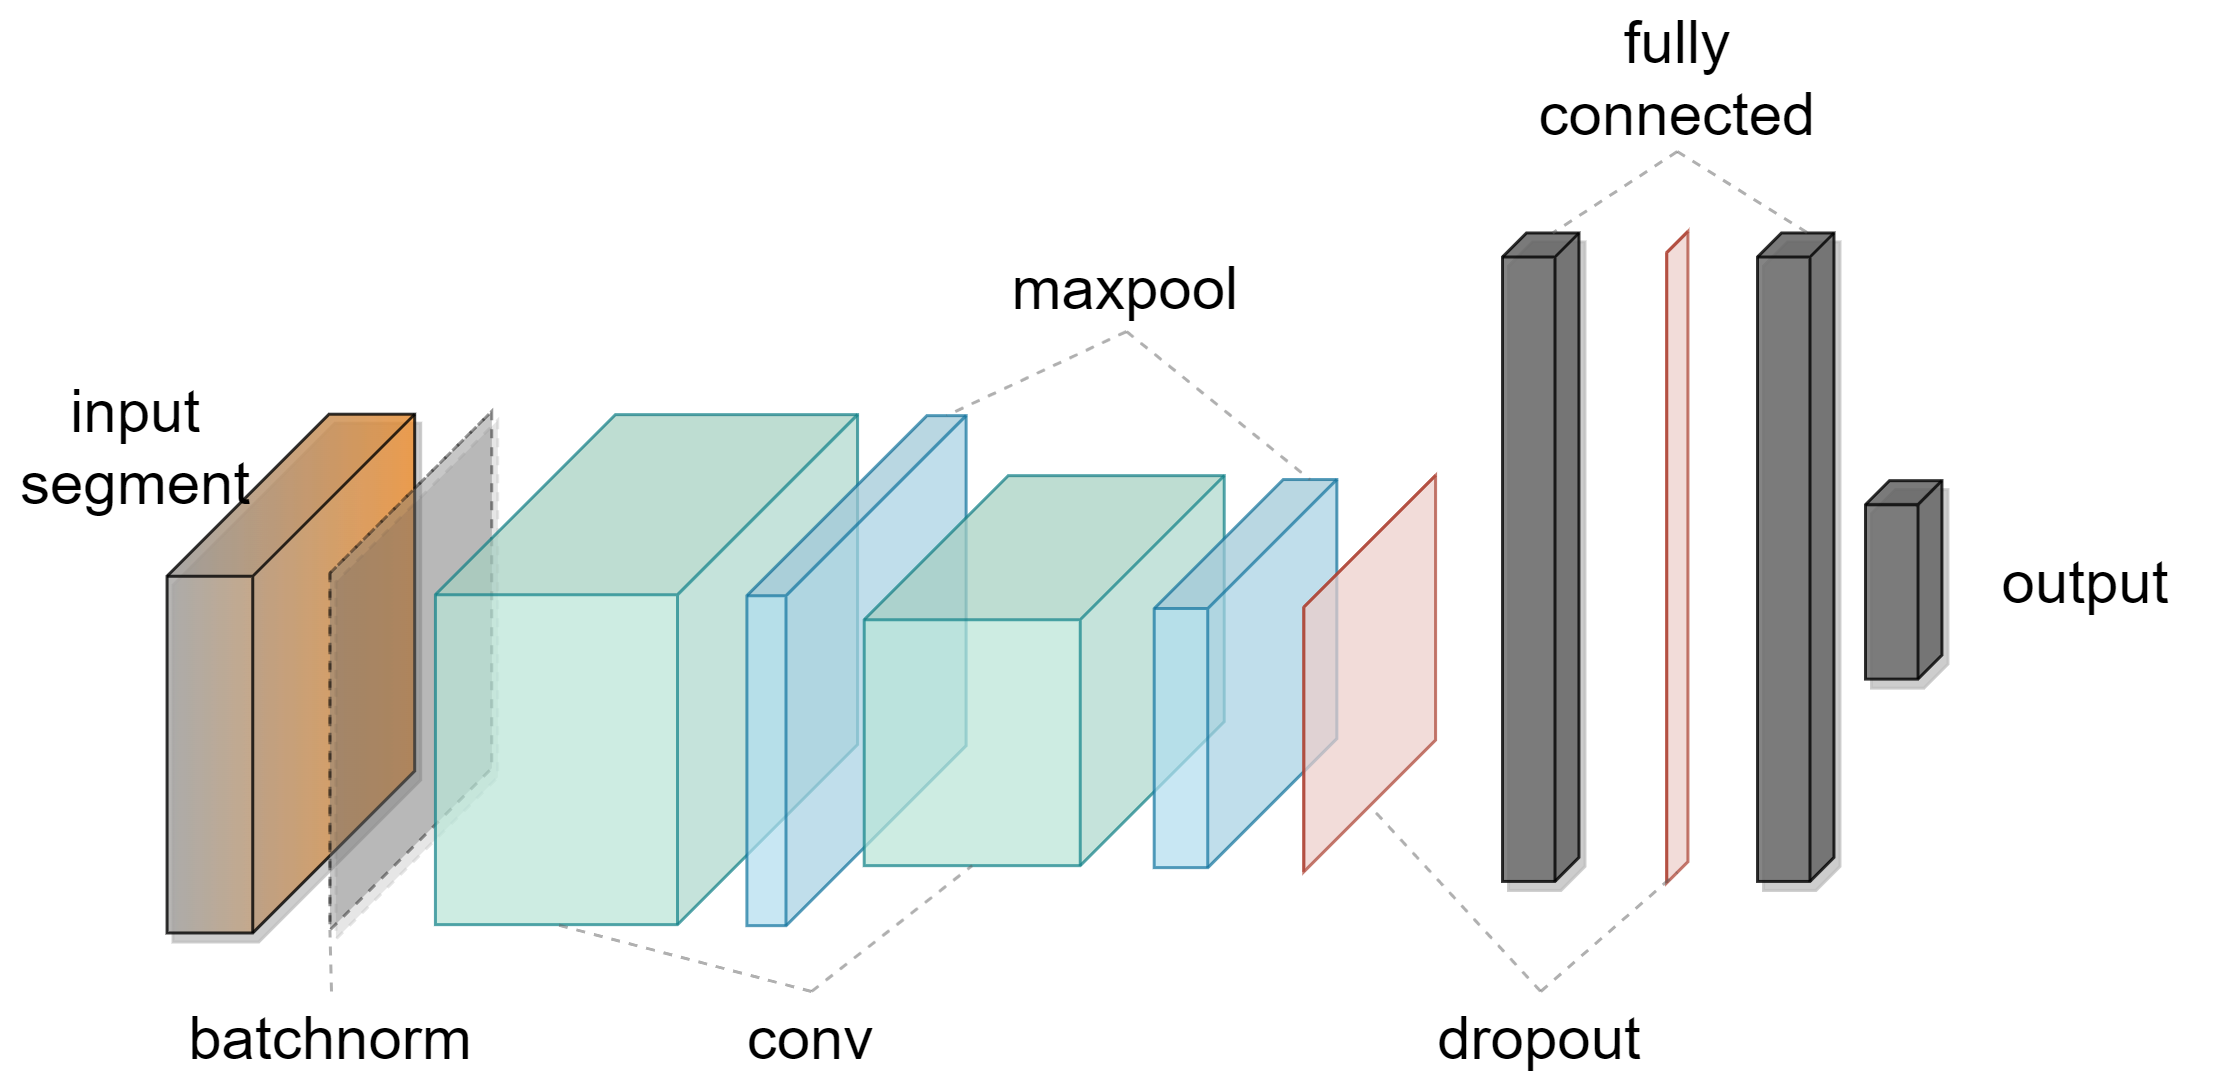
\includegraphics[width=\linewidth]{\subdir/CNN.drawio.png}
    \caption[Model architecture]{Convolutional Neural Network
        \nameref{subsec:model-architecture} used in this work. Different layer
        sizes are used as well as different input segment dimensions. The
        output of the last fully connected layer changes with the model
        \nameref{subsec:model-task} too.}
    \label{fig:model-arch-cnn}
\end{figure}

\subsubsection{Task} \label{subsec:model-task}

One can find here a description of the different tasks implemented and tested
in models. Tasks define the goal of the model and the way its loss is computed.

\paragraph{Classification} \label{para:model-task-class} Consists in
classifying the longitudinal velocity given a set of possibilities. The
different classes are ranges of longitudinal velocities, being these ranges a
hyperparameter of the model. Cross entropy loss is computed between the
predicted class probabilities and the class corresponding to the target
longitudinal velocity and the predicted class. The output of the model is
therefore a vector of probabilities corresponding to each class.

\paragraph{Ordinal classification} \label{para:model-task-ord-class} Consists
in classifying the longitudinal velocity given a set of possibilities like in
\nameref{para:model-task-class}, with different classes being ranges of
longitudinal velocities. But the order of the class matters. This method was
introduced in \cite{ordclass2006}, where standard classification algorithms are
extended to make use of the order of the classes. The output of this model is a
vector of binary values that can be decoded into a class position by making use
of a ranking rule. The loss is computed with the mean square error between the
target class position and the predicted class position. 

\subsubsection{Architecture} \label{subsec:model-architecture}

This section describes the different model architectures implemented and
evaluated. A common point of them all is simplicity. It is out of the scope of
this work to find an optimal architecture for acoustic odometry. But it is
interesting to evaluate different simple options.

\paragraph{CNN with normalized input} \label{para:model-arch-norm-cnn} This
architecture is identical to the \nameref{para:model-arch-cnn} except for the
fact that it contains a batch normalization layer \cite{batchnorm2015} as shown
in \cref{fig:model-arch-cnn}.

\begin{table}
    \centering
    \begin{tabular}{|c|c|c|c|c|c|c|}
        \hline
        \multirow{2}{*}{Name}
                      & \multicolumn{2}{c|}{Conv 1}

        
        
                      & \multicolumn{2}{c|}{Conv 2}

        
        
                      & \multirow{2}{*}{Hidden units}

        
        
                      & \multirow{2}{*}{Size [MB]}                                              \\
        \cline{2-5}
                      & Filters                       & Kernel & Filters & Kernel &     &       \\
        \hline
        \hline
        \texttt{base} & 64                            & 5      & 128     & 5      & 512 & 412.6 \\\hline
        \texttt{M}    & 32                            & 5      & 64      & 5      & 256 & 103.2 \\\hline
        \texttt{S}    & 16                            & 5      & 32      & 5      & 256 & 51.5  \\\hline
        \texttt{XS}   & 8                             & 5      & 16      & 5      & 128 & 12.9  \\\hline
        \texttt{XXS}  & 4                             & 3      & 8       & 3      & 64  & 3.4   \\\hline
        \texttt{XXXS} & 2                             & 3      & 4       & 3      & 32  & 0.87  \\\hline
    \end{tabular}
    \caption[Model sizes]{Different sizes used for the model
        \nameref{subsec:model-architecture} in this work. \emph{Conv 1}
        corresponds to the first convolutional layer, \emph{Conv 2} to the
        second. \emph{Hidden units} corresponds to the units between the two
        last fully connected layers. The input of the first fully connected
        layer is determined by the output elements of the second convolutional
        layer while the output of the second fully connected layer is
        determined by the model \nameref{subsec:model-task}. Sizes in megabytes
        correspond to models with input segments of 120 frames with 256
        features from 1 extractor and classification output with 7 classes. }
    \label{table:model-arch-sizes}
\end{table}

% Squeeze-net